\ifdefined\included
\else
\documentclass[english,a4paper,11pt,twoside]{StyleThese}
\usepackage{amsmath,amssymb}             % AMS Math
\usepackage[T1]{fontenc}
\usepackage[utf8x]{inputenc}
\usepackage{babel}
\usepackage{datetime}

\usepackage{lmodern}
\usepackage{tabularx}
%\usepackage{tabular}
\usepackage{multirow}

\usepackage{subfigure}
\usepackage{fancyvrb}
\usepackage{algorithmic}
\usepackage{algorithm}
\usepackage{mathtools}


\usepackage{hhline}
\usepackage[left=1.5in,right=1.3in,top=1.1in,bottom=1.1in,includefoot,includehead,headheight=13.6pt]{geometry}
\renewcommand{\baselinestretch}{1.05}

% Table of contents for each chapter

\usepackage[nottoc, notlof, notlot]{tocbibind}
\usepackage{minitoc}
\setcounter{minitocdepth}{2}
\mtcindent=15pt
% Use \minitoc where to put a table of contents

\usepackage{aecompl}


% Glossary / list of abbreviations

\usepackage[intoc]{nomencl}
\iftoggle{ThesisInEnglish}{%
\renewcommand{\nomname}{Glossary}
}{ %
\renewcommand{\nomname}{Liste des Abréviations}
}

\newcommand{\accom}[1]{\textcolor{red}{[#1]}}

\makenomenclature

% My pdf code

\usepackage{ifpdf}

\ifpdf
  \usepackage[pdftex]{graphicx}
  \DeclareGraphicsExtensions{.jpg}
  \usepackage[a4paper,pagebackref,hyperindex=true]{hyperref}
  \usepackage{tikz}
  \usetikzlibrary{arrows,shapes,calc}
\else
  \usepackage{graphicx}
  \DeclareGraphicsExtensions{.ps,.eps}
  \usepackage[a4paper,dvipdfm,pagebackref,hyperindex=true]{hyperref}
\fi

\graphicspath{{.}{images/}}

%% nicer backref links. NOTE: The flag ThesisInEnglish is used to define the
% language in the back references. Read more about it in These.tex

\iftoggle{ThesisInEnglish}{%
\renewcommand*{\backref}[1]{}
\renewcommand*{\backrefalt}[4]{%
\ifcase #1 %
(Not cited.)%
\or
(Cited in page~#2.)%
\else
(Cited in pages~#2.)%
\fi}
\renewcommand*{\backrefsep}{, }
\renewcommand*{\backreftwosep}{ and~}
\renewcommand*{\backreflastsep}{ and~}
}{%
\renewcommand*{\backref}[1]{}
\renewcommand*{\backrefalt}[4]{%
\ifcase #1 %
(Non cité.)%
\or
(Cité en page~#2.)%
\else
(Cité en pages~#2.)%
\fi}
\renewcommand*{\backrefsep}{, }
\renewcommand*{\backreftwosep}{ et~}
\renewcommand*{\backreflastsep}{ et~}
}

% Links in pdf
\usepackage{color}
\definecolor{linkcol}{rgb}{0,0,0.4} 
\definecolor{citecol}{rgb}{0.5,0,0} 
\definecolor{linkcol}{rgb}{0,0,0} 
\definecolor{citecol}{rgb}{0,0,0}
% Change this to change the informations included in the pdf file

\hypersetup
{
bookmarksopen=true,
pdftitle="Joint Action for Human-Robot Interaction",
pdfauthor="Sandra DEVIN", %auteur du document
pdfsubject="Thesis", %sujet du document
%pdftoolbar=false, %barre d'outils non visible
pdfmenubar=true, %barre de menu visible
pdfhighlight=/O, %effet d'un clic sur un lien hypertexte
colorlinks=true, %couleurs sur les liens hypertextes
pdfpagemode=None, %aucun mode de page
pdfpagelayout=SinglePage, %ouverture en simple page
pdffitwindow=true, %pages ouvertes entierement dans toute la fenetre
linkcolor=linkcol, %couleur des liens hypertextes internes
citecolor=citecol, %couleur des liens pour les citations
urlcolor=linkcol %couleur des liens pour les url
}

% definitions.
% -------------------

\setcounter{secnumdepth}{3}
\setcounter{tocdepth}{2}

% Some useful commands and shortcut for maths:  partial derivative and stuff

\newcommand{\pd}[2]{\frac{\partial #1}{\partial #2}}
\def\abs{\operatorname{abs}}
\def\argmax{\operatornamewithlimits{arg\,max}}
\def\argmin{\operatornamewithlimits{arg\,min}}
\def\diag{\operatorname{Diag}}
\newcommand{\eqRef}[1]{(\ref{#1})}

\usepackage{rotating}                    % Sideways of figures & tables
%\usepackage{bibunits}
%\usepackage[sectionbib]{chapterbib}          % Cross-reference package (Natural BiB)
%\usepackage{natbib}                  % Put References at the end of each chapter
                                         % Do not put 'sectionbib' option here.
                                         % Sectionbib option in 'natbib' will do.
\usepackage{fancyhdr}                    % Fancy Header and Footer

% \usepackage{txfonts}                     % Public Times New Roman text & math font
  
%%% Fancy Header %%%%%%%%%%%%%%%%%%%%%%%%%%%%%%%%%%%%%%%%%%%%%%%%%%%%%%%%%%%%%%%%%%
% Fancy Header Style Options

\pagestyle{fancy}                       % Sets fancy header and footer
\fancyfoot{}                            % Delete current footer settings

%\renewcommand{\chaptermark}[1]{         % Lower Case Chapter marker style
%  \markboth{\chaptername\ \thechapter.\ #1}}{}} %

%\renewcommand{\sectionmark}[1]{         % Lower case Section marker style
%  \markright{\thesection.\ #1}}         %

\fancyhead[LE,RO]{\bfseries\thepage}    % Page number (boldface) in left on even
% pages and right on odd pages
\fancyhead[RE]{\bfseries\nouppercase{\leftmark}}      % Chapter in the right on even pages
\fancyhead[LO]{\bfseries\nouppercase{\rightmark}}     % Section in the left on odd pages

\let\headruleORIG\headrule
\renewcommand{\headrule}{\color{black} \headruleORIG}
\renewcommand{\headrulewidth}{1.0pt}
\usepackage{colortbl}
\arrayrulecolor{black}

\fancypagestyle{plain}{
  \fancyhead{}
  \fancyfoot{}
  \renewcommand{\headrulewidth}{0pt}
}

%\usepackage{MyAlgorithm}
%\usepackage[noend]{MyAlgorithmic}
\usepackage[ED=MITT - STICIA, Ets=INP]{tlsflyleaf}
%%% Clear Header %%%%%%%%%%%%%%%%%%%%%%%%%%%%%%%%%%%%%%%%%%%%%%%%%%%%%%%%%%%%%%%%%%
% Clear Header Style on the Last Empty Odd pages
\makeatletter

\def\cleardoublepage{\clearpage\if@twoside \ifodd\c@page\else%
  \hbox{}%
  \thispagestyle{empty}%              % Empty header styles
  \newpage%
  \if@twocolumn\hbox{}\newpage\fi\fi\fi}

\makeatother
 
%%%%%%%%%%%%%%%%%%%%%%%%%%%%%%%%%%%%%%%%%%%%%%%%%%%%%%%%%%%%%%%%%%%%%%%%%%%%%%% 
% Prints your review date and 'Draft Version' (From Josullvn, CS, CMU)
\newcommand{\reviewtimetoday}[2]{\special{!userdict begin
    /bop-hook{gsave 20 710 translate 45 rotate 0.8 setgray
      /Times-Roman findfont 12 scalefont setfont 0 0   moveto (#1) show
      0 -12 moveto (#2) show grestore}def end}}
% You can turn on or off this option.
% \reviewtimetoday{\today}{Draft Version}
%%%%%%%%%%%%%%%%%%%%%%%%%%%%%%%%%%%%%%%%%%%%%%%%%%%%%%%%%%%%%%%%%%%%%%%%%%%%%%% 

\newenvironment{maxime}[1]
{
\vspace*{0cm}
\hfill
\begin{minipage}{0.5\textwidth}%
%\rule[0.5ex]{\textwidth}{0.1mm}\\%
\hrulefill $\:$ {\bf #1}\\
%\vspace*{-0.25cm}
\it 
}%
{%

\hrulefill
\vspace*{0.5cm}%
\end{minipage}
}

\let\minitocORIG\minitoc
\renewcommand{\minitoc}{\minitocORIG \vspace{1.5em}}

\usepackage{multirow}
%\usepackage{slashbox}

\newenvironment{bulletList}%
{ \begin{list}%
	{$\bullet$}%
	{\setlength{\labelwidth}{25pt}%
	 \setlength{\leftmargin}{30pt}%
	 \setlength{\itemsep}{\parsep}}}%
{ \end{list} }

\newtheorem{definition}{Définition}
\renewcommand{\epsilon}{\varepsilon}

% centered page environment

\newenvironment{vcenterpage}
{\newpage\vspace*{\fill}\thispagestyle{empty}\renewcommand{\headrulewidth}{0pt}}
{\vspace*{\fill}}

\usepackage{tablefootnote}

\sloppy
\begin{document}
\setcounter{chapter}{3} %% Numéro du chapitre précédent ;)
\dominitoc
\faketableofcontents
\fi

\chapter{When to take decisions during Shared Plans elaboration and execution}
\minitoc

\label{ch:SP}

\section{Motivation}

When performing a Joint Action and more particularly when executing Shared Plans, several choices have to be made. Some of them are implicit, while others require a negotiation or an adaptation between the Joint Action participants. To be a good partner when performing Joint Action with humans, the robot should be able to identify which decisions are implicit and correctly communicate about the other ones. Indeed, a robot which communicates about each detail of a Shared Plan would easily become too "chatty" when a robot which does not communicate can be confusing.

Let's take for example a robot helping a human to build a flat-pack table: the legs of the table need to be assembled with a hammer, the tray with a screwdriver and finally someone needs to put the tray on the legs. The robot is equipped with several tools including a screwdriver but no hammer and the human has only one hammer. The human and the robot are both able to put the tray on the legs. It is common sense that the robot should assemble the tray while the human assemble the legs. However, a decision needs to be taken concerning who will put the tray on the legs. 
In this scenario, the robot should assemble the tray without asking the human and negotiate or adapt its behavior to put the tray. 

The work presented in this chapter consists in finding which decisions are implicit or not, when the decisions should be taken and how to take them. We identify three types of decisions to be taken during Shared Plans elaboration and execution:
\begin{itemize}
\item \textbf{Which action to perform in which order:} this is one of the biggest concern during Shared Plan elaboration. We do not focus our work in this part. Indeed, we use for this part HATP, a human-aware HTN planner which has been demonstrated to be well suited to human-robot joint action \cite{Lallement2014hatp}.
\item \textbf{Who will perform which action:} sometimes this decision can be implicit when only one agent is able to perform an action. However, in other situations, the robot should be able to decide who will perform an action by negotiating or adapting its behavior to the human one.
\item \textbf{With which object:} for practical reason, the robot reasons on objects by attributing them a unique id. However, for the purpose of an action, two objects can be semantically identical. When there is a choice in which object to use for an action, the robot should be able to adapt to the human behavior in order to avoid potential conflicts.
\end{itemize}

\section{Background}

When the robot needs to achieve a joint goal, several works allow it to compute plans which take into account the human (\cite{cirillo2010human,Lallement2014hatp}). They allow the robot to reduce resource conflicts \cite{chakraborti2016planning}, take divergent beliefs into account (\cite{guitton2012belief,talamadupula2014coordination}) or promote stigmergic collaboration
for agents in co-habitation \cite{chakraborti2015planning}. 

The relevance of using a Shared Plan in human-robot interaction has been studied by \cite{lallee2013cooperative}. They suggest that the joint plan should be fully communicated in order to sustain effective collaboration. Moreover, in \cite{gombolay2015decision}, it is shown that subjects prefer letting the robot plan when the task is too complex, prioritizing efficiency. 
In more simple tasks, a robot proactively helping the human is preferred to one waiting before proposing help \cite{baraglia2016initiative}. 

If the robot decides to share the plan, several studies have been reported on how to do communicate about the plan. Some researchers studied how a system could acquire knowledge on plan decomposition from a user \cite{Mohseni2015} and how dialog can be used to teach new collaborative plans to the robot and to modify these plans \cite{petit2013coordinating}. In \cite{sorce2015proof}, the system is able to learn a plan from a user and transmit it to another user. \cite{allen2002human} presents a computer agent able to construct a plan in collaboration with a user. Finally, in \cite{milliez2016using}, Milliez et al. present a system where the robot shares the plan with a level of details which depends on the expertise of the user. In our work, we try to get rid of the entire shared plan verbalization by taking the right decision at the right time in order to come up with a robot which communicates at the right time.

Several contributions have been done to allow more adaptability during shared plan execution. \cite{chien2000using} proposes a method to plan only a few steps in advance and then plan the actions further in an iterative way. Chaski, a task-level
executive, presented in \cite{shah2011improved}, allows to choose when to execute the robot actions adapting to a human partner. A system which mixes plan recognition and adaptation is described in \cite{levine2014concurrent}. It computes all possibilities for the plan and chooses an action based on the choice of the human and causal links. \cite{hoffman2007effects} proposes an adaptive action selection mechanism for a robotic teammate, making anticipatory decisions based on the confidence of their validity and their relative risk. \cite{karpas2015robust} presents Pike, an online executive that unifies intent recognition and plan adaptation for temporally flexible plans with choice. Finally, this work is based on SHARY \cite{clodic2009shary} which was extended in \cite{fiore2014planning}, a supervisor allowing to execute human-aware shared plans taking into account joint actions aspects like reactive action execution.

In the cooperative multi-robot literature, task allocation and cooperative activity achievement has been thoroughly investigated \cite{gerkey2004formal}. Auction has been used very successfully for distributed multi-robot in various contexts (\cite{gerkey2002sold,botelho1999m+}). 
Concerning the so-called teamwork and cooperative task achievement taking into account explicit constraints to facilitate the activity of the other robots or agents activity, one can mention \cite{tambe1997agent} and \cite{joyeux2009plan}. While these contributions have inspired work on human-robot collaboration, it is however important to exhibit some differences between the two fields. Indeed, the human and the robot are not equal in any aspect. The robot is here to help the human and facilitate his activity.

In AI, the goal reasoning domains deals with some problems similar to Shared Plan management \cite{molineaux2010goal, roberts2016goal}. The role of goal reasoning is to survey the current goals of a robot, check that they remain feasible and relevant and establish new goals if needed. Moreover, part of the goal reasoning function is sometimes linked to the plan management as it is in charge of deciding when and how to generate plans (but it is not producing the plan) and checking for unexpected events. 

\section{Assumptions}

The work presented in this chapter treats of the needed decision during Shared Plan elaboration and execution. The focus is put here into the decisions concerning the action allocation and instantiation. To do so, we make several assumptions:

\paragraph{Single human:} the work presented in this chapter has been designed for a robot interacting with a single human. However, all the data structures and main principles are compatible with multi-humans set-up.

\paragraph{Commitment:} we do not focus in this works on issues related to commitment. Consequently, we consider here that the joint goal has already been established. We also consider that the human will not abort the goal unless he knows that the goal is not achievable any more.

\paragraph{Shared Plan:} we put the focus here on the issues related to action allocation and instantiation. In order to decide which action to execute in which order, we use HATP, a human-aware HTN planner which has been demonstrated to be well suited to human-robot Joint Action \cite{Lallement2014hatp}.
We are focusing in this work about medium complexity Shared Plans where the human might want to decide for his own actions.

\paragraph{Humans perception:} we make the assumption here that a human will see and understand an action of the robot when he is present and looking at it. We also assume that when he is present, the human is able to hear and understand the information verbalized by the robot.

\paragraph{Robot capacities:} we consider that the robot is able to perform simple high level actions like Pick, Place or Drop. We also assume that the robot is able to ask to the human if he wants to perform an action and to understand a basic answer (yes/no type). 
The robot is able to detect and localize objects and agents
and to recognize simple high level actions performed by the human like Pick, Place or Drop. Let us also note that the ways the robot achieves actions (e.g. human-aware motion planning and execution) and recognizes human's actions are outside of the scope of this chapter.

\paragraph{Communication:} the focus of this work is more on the what to communicate and when than on the how to communicate. Here we use the basic dialogue module described in Chapter~\ref{ch:Sup} to communicate with the human but more complex communication mechanisms can be envisioned. 

\section{Main principles}

We will present in this section the main principles we use for Shared Plans management. Three algorithms are used to allow the robot to elaborate and execute Shared Plans.  They interact through the Shared Plan data \textit{SP} and several signals (noted \textit{S\_X} where \textit{X} is the name of the signal). These three algorithm run constantly and in parallel.They allow respectively to maintain the state of the shared plan, to choose actions for the robot, and to monitor the human.

The Alg.~\ref{alg:mainPlan} allows the robot to elaborate a Shared Plan when needed, to maintain the current Shared Plan and to manage the human mental states. The terms used in the algorithms are reminded in Appendix \ref{chap:annexe1}.

\begin{algorithm}
\caption{Shared Plan management}
\label{alg:mainPlan}
\begin{algorithmic}
\WHILE {$g_R$}
\IF {$!SP \ \| \ S\_needReplan$}
\STATE $SP \leftarrow PLAN(g_R, WS)$
\ENDIF
\IF {S\_needUpdate}
\STATE $SP \leftarrow UPDATE\_PLAN(SP, WS)$
\ENDIF
\IF {S\_actionAllocated}
\STATE $SP \leftarrow EVALUATE\_ PLAN(SP, WS)$
\ENDIF
\IF {$Obj_g \in WS$ \hfill \textit{$\vartriangleright$ The goal is achieved}
\STATE}
\STATE $g_R \leftarrow \emptyset$ 
\STATE $SP \leftarrow \emptyset$
\ENDIF
\IF {$<Human, isPresent, true> \in WS \ \& \ (WS(H) \neq WS(H)_{t-1} \  \|  \  TS \neq TS_{t-1})$}
\STATE $MS(H) \leftarrow ESTIMATE\_MS(MS(H), TS)$
\IF {$MS(H) \neq TS$ \hfill \textit{$\vartriangleright$ Divergent belief}
\STATE}
\STATE $SOLVE\_DB(MS(H), TS)$
\ENDIF
\ENDIF
\ENDWHILE
\end{algorithmic}
\end{algorithm} 

When the robot has a goal $g_R$ to achieve and no current plan or when a signal is received to compute a new plan ($S\_needReplan$), the robot computes a Shared Plan to perform the goal based on the current world state $WS$ (see Sec.~\ref{sec:elaboration}):
$$SP \leftarrow PLAN(g_R, WS)$$

When an action $a$ from the plan is performed by an agent a signal is received ($S\_needUpdate$) and the robot updates the plan (see Sec.~\ref{subsec:maintaining}):
$$SP \leftarrow UPDATE\_PLAN(SP, a)$$

When an action from $A^X$ has been allocated ($S\_actionAllocated$), the robot looks for the consequences of this allocation in the plan (see Sec.~\ref{subsec:allocation}):
$$SP \leftarrow EVALUATE\_ PLAN(SP, WS)$$
The robot also constantly checks if the goal is reached (the objectives of the goal are in the current World State).
Finally, each time a change occurs in $WS(H)$ or $TS$, the robot estimates the human mental states as described in the previous chapter (see Chapter~\ref{ch:MS}):
$$MS(H) \leftarrow ESTIMATE\_MS(MS(H), TS)$$
If there is a conflict between the knowledge of the robot and the human mental state, the robot tries to solve it (see Chapter~\ref{ch:MS}): 
$$SOLVE\_DB(MS(H), TS)$$

In parallel to the first algorithm, Alg.~\ref{alg:mainExec} allows the robot to decide when to act and which action to perform. 


\begin{algorithm}
\caption{Robot action decision}
\label{alg:mainExec}
\begin{algorithmic}
\WHILE {$SP$}
\STATE $A_{next} \leftarrow GET\_NEXT\_ACTIONS(SP, WS)$
\IF {$A_{next} = \emptyset$ \hfill \textit{$\vartriangleright$ No more feasible actions}
\STATE}
\STATE $S\_needReplan$
\ELSIF {$\{A^R_{next} \cup A^X_{next}\} =  \emptyset$ \hfill \textit{$\vartriangleright$ No actions for the robot
\STATE}}
\STATE $actionExecuted \leftarrow WAIT\_ACTION(A^H_{next}, t)$
\IF {!actionExecuted}
\STATE $S\_needReplan$
\ENDIF 
\ELSE
\STATE $a \leftarrow SELECT\_ACTION\_TODO(A_{next})$
\IF {$a \in A^X_{next}$}
\STATE $actor \leftarrow ALLOCATE\_ACTION(SP, a, WS, Prefs)$
\STATE $S\_actionAllocated$
\ENDIF
\IF {$a \in A^R_{next} \ \| \ (a \in A^X_{next} \ \& \ actor = robot)$}
\STATE $success \leftarrow EXECUTE(a)$
\IF {success}
\STATE $S\_needUpdate$
\ELSE 
\STATE $S\_needReplan$
\ENDIF
\ELSIF {$(a \in A^X_{next} \ \& \ actor = human)$}
\STATE $a \rightarrow A^H_{next}$
\ENDIF
\ENDIF
\ENDWHILE
\end{algorithmic}
\end{algorithm} 

When the robot has a Shared Plan $SP$, it looks for the action of this plan which need to and can be executed (see Sec. \ref{subsec:maintaining}):
$$A_{next} \leftarrow GET\_NEXT\_ACTIONS(SP, WS)$$
If there is no action in $A_{next}$ nor in progress, it means that the plan is blocked, so the robot looks for another Shared Plan. If there are actions to do, the robot looks if there is an action it can execute (actions allocated to it or not allocated yet). If there is none, the robot waits for the human to perform an action ($A_{next}$ contains only actions from $A^H_{next}$):
$$actionExecuted \leftarrow WAIT\_ACTION(A^H_{next}, t)$$
If after a time \textit{t}, the human did not execute any action, the robot looks for another plan.
If there are actions the robot can execute, the robot selects an action $a$ (see Sec. \ref{subsec:selection}):
$$a \leftarrow SELECT\_ACTION\_TODO(A_{next})$$
If the selected action is not yet allocated, the robot first tries to allocate it (see Sec. \ref{subsec:allocation}):
$$actor \leftarrow ALLOCATE\_ACTION(SP, a, WS, Prefs)$$
If the action is allocated to the robot (after selection or allocation), the robot executes it:
$$success \leftarrow EXECUTE(a)$$
It will first instantiate the action if needed and then launch its execution (see Sec. \ref{subsec:execution}). If the action succeeds, the robot updates the plan, else it looks for another plan.

In parallel to the other execution loops, the robot is constantly monitoring human activities (Alg.~\ref{alg:monitoring}).

\begin{algorithm}
\caption{Human monitoring}
\label{alg:monitoring}
\begin{algorithmic}
\WHILE {$<Human, isPresent, true> \in WS$}
\IF {$\exists \ a \in A^H_{cur}$}
\IF {$a \in A^R_{cur}$}
\STATE $S\_stop$
\ENDIF
\STATE WAIT\_END\_ACTION(a)
\IF {$a \in A^H_{next}$}
\STATE $S\_needUpdate$
\ELSIF {$a \in A^X_{now}$}
\STATE $S\_actionAllocated$
\ELSE 
\STATE $S\_needReplan$ \hfill \textit{$\vartriangleright$ Unexpected action}
\ENDIF
\ENDIF
\ENDWHILE
\end{algorithmic}
\end{algorithm}

When the human performs an action, the robot first looks if the action is concurrent to the one it is performing (for example, if the human picks an object the robot was going to pick), and if it is the case, the robot stops its actions.  
Then, if the human performs an expected action with respect to the plan and already allocated to him, the robot updates the plan accordingly. If the action executed by the human is expected with respect to the plan but was not yet allocated, the robot looks for the consequences of this actions in the plan (see Sec. \ref{subsec:allocation}).
If the human performs an unexpected action with respect to the plan (action not in $A_{next}$ or in $A^R_{next}$), the robot looks for a new plan from the new situation induced by the human action.

The next sections will define more precisely the operators we just defined.


\section{Shared Plans elaboration}

\label{sec:elaboration}

The first step of this work is to be able to compute Shared Plans flexible enough to let part of the decisions to execution time. This step correspond to the operator:
$$PLAN(g_R, WS)$$

As stated before, the human-aware HTN task planner HATP is used in this work to compute Shared Plans taking into account a number of social rules for both the robot and its human partner \cite{Lallement2014hatp}. However, in order to obtain flexible plans with HATP, a number of issues have to be considered.

First, when HATP returns a plan, it returns only one, which is assumed to be the best plan it has found given the situation and the associated costs. However, this plan is not always the only one possible (even at constant cost or computing time). Indeed, in such case, HATP makes some choices that could be preferably done on-line. For example, it can happen that one action can be done by several agents at the same cost. In a collaborative setting and more particularly when the human is concerned, it could be interesting to let the agents decide at execution time (or whenever it is interesting) who will do what. To handle this, we have adapted HATP by inserting what we call the\textit{X agent}. The capabilities of the \textit{X agent} correspond to the intersection of the capabilities of the human and the robot with a lower cost. Consequently, it will be chosen by the planner instead of the human or the robot whenever it is possible. If HATP returns a plan containing an action to be done by the \textit{X agent}, it means that this action could either be performed by the human or the robot. The decision concerning who will finally do this action is postponed. We will see in Sec. \ref{subsec:allocation} how \textit{X agent} actions will be finally allocated to the human or the robot.

As inputs to a planner such as HATP, we give a set of objects that are present in the environment and on which it will be able to apply its operators. Basically, each object is tagged and is unique. That means that if we have the same object twice, they will be uniquely tagged (e.g. two identical red cubes will be tagged as RED\_CUBE\_1 and RED\_CUBE\_2). When two similar objects can be used in a same way during a task, the planner will choose either one or the other. In a collaborative setting, it could be counter intuitive since even if there is no distinction between the two objects at planning time, there can be one during execution. To handle this, we have adapted HATP by inserting the notion of \textit{similar} objects which aims to group interchangeable objects under a common name: two \textit{similar} objects will have the same role in the task. 

Finally, rather than in other works where we used HATP, we do not consider here that an agent is only capable to perform one action at a time. This allows the human to choose the order of his action when there is no impact in the global plan.

\section{Shared Plans execution}

We will now see in more detail how the robot executes the flexible Shared Plans obtained.

\subsection{Plan maintaining}
\label{subsec:maintaining}

First, the robot needs to be able to follow the Shared Plan execution and to determine which actions need to be executed and which actions need to be left for later. 

As said before, the actions composing a Shared Plan can be decomposed as:
$$A_p = <A_{prev}, A_{cur}, A_{next}, A_{later}>$$

By default, when a Shared Plan is computed by the robot, all actions are put in $A_{later}$. When the robot performs an action or detects an action execution from a human, the executed action goes in $A_{cur}$ and, at the end of the execution, the action goes in $A_{prev}$ with a label equal either to DONE if the execution has been successful, FAILED if not or ABORTED if the robot had to stop the execution for an external reason.

An action will be put in $A_{next}$ if all previous actions in the plan are DONE (based on causal links) and its preconditions are checked:

$$a \in A_{next} \Leftrightarrow Precs_{a} \in WS \ \& \ (\forall l \in L_p \ | \ next_l = id_a,$$ 
$$\exists \ ap \in A_{prev} \ | \ (id_{ap} = prev_l \ \& \ label_{ap}  = DONE))$$

The $UPDATE\_PLAN$ operator updates the state of each action of the plan and the $GET\_NEXT\_ACTIONS$ operator returns the actions in $A_{next}$.


\subsection{Action selection}
\label{subsec:selection}

Once the robot knows which actions need to be executed, it needs to choose one from the set of actions it can execute. To do so, it uses the $SELECT\_ACTION\_TODO$ operator which returns the action with the higher priority:

$$\underset{a \in \{A^R_{next} \cup A^X_{next}\}}{\mathrm{argmax}} \ priority(a)$$

\textbf{Priorities used:}
In our case, we have chosen to give higher priority to the actions allocated to the robot compared to those not already allocated. In general for this work, we have made the choice to postpone as much as possible the decisions made by the robot. Indeed, this choice is made in order to give as much latitude as possible to the human, which allows him to take the initiative until the last possible moment. In the current implementation of our system, the priorities of the different actions of the robot are the same, so the robot will simply select one. However, there is a possibility to later integrate costs as, for example, select the action the farthest of what the human is currently doing. Concerning the priorities of not allocated actions, we still follow the principle to postpone as much as possible the robot decision. To do so, we put a higher priority on what we call \textit{analogous} actions. Two actions will be \textit{analogous} when they have exactly the same decomposition (same action name and same parameters). Indeed, as there is several time the action to execute, putting a higher priority on \textit{analogous} actions allows to robot to execute one (and advance in the plan) while letting to the human the possibility to perform the other one.

\subsection{Action allocation}
\label{subsec:allocation}

Once a not yet allocated action is selected, the robot needs to decide if it should execute it or not ($ALLOCATE\_ACTION$ operator). To do so, the robot first looks for the possible actors of this action: agents which verify the preconditions of the action and which are not already busy. Note that even if the action was not allocated by HATP it is possible that there is only one possible actor. In this case, the robot automatically allocates the action to this agent. For example if the human is currently busy and there is a not allocated action  to perform, the robot will execute it. If there is more than one possible actor for the action, the robot follows the algorithm \ref{alg:allocate}.

\begin{algorithm}
\caption{Action allocation: $SP \leftarrow ALLOCATE\_ACTION(SP, a, WS, Prefs)$}
\label{alg:allocate}
\begin{algorithmic}
\REQUIRE $a \in A^X_{next}$
\IF {$cost(a, R) << cost(a, H)$}
\STATE $actor \leftarrow robot$
\ELSIF {$cost(a, H) << cost(a, R)$}
\STATE $actor \leftarrow human$
\ELSIF {mode = negotiation}
\STATE $answer \leftarrow ASK(a, H)$
\IF {answer = yes}
\STATE $actor \leftarrow human$
\ELSE
\STATE $actor \leftarrow robot$
\ENDIF
\ELSE
\STATE $actionPerformed \leftarrow WAIT\_ACTION(a, t)$
\hfill \textit{$\vartriangleright$ adaptation mode}
\IF {$actionPerformed$}
\STATE $actor \leftarrow human$
\ELSE
\STATE $actor \leftarrow robot$
\ENDIF
\ENDIF
\RETURN $actor$
\end{algorithmic}
\end{algorithm}

First, the robot compares the estimated cost for the human and for itself to perform the action. If it considers it significantly more costly for the human to perform the action, it will allocate the action to itself. Then, we have developed two possible modes for the robot. In the first mode, called \textbf{negotiation} mode, the robot directly asks its human partner if he wants to perform the action and then allocates the action according to his answer. In the other mode, called \textbf{adaptation} mode, the robot waits a certain amount of time, and, if the human does not take the initiative to perform the action, it executes it. 

Allocating an action to an agent can lead to other actions being automatically allocated. For this reason, after each allocation of an action, a new plan is built taking into account the possible allocations of the actions remaining in $A_X$.

\textbf{Costs used for action selection ($cost(a, R)$ and $cost(a, H)$):}
In the current implementation, we use a cost concerning the \textit{analogous} actions (see description in the previous subsection). These \textit{analogous} actions will have a lower cost for the robot to execute them leading the robot to automatically execute one of them. Indeed, as there is several time the same action to perform, the robot can execute one while letting to the human the possibility to perform the other(s).

Other costs can be considered as human preferences. We can imagine having a list of actions the human likes to perform and another he dislikes. The robot can then allocate the actions following these preferences.

\subsection{Action execution}
\label{subsec:execution}

Once the robot has decided to execute an action ($EXECUTE$ operator), it needs to be able to deal with the \textit{similar} objects introduced before. To do so, we keep the principle that the robot waits until the last moment to take a decision. For example, if the robot and the human have to pick objects and place them in several similar placements, the robot will first pick an object and only after choose a placement to place it. Then, when the robot has to choose an object, it will choose the one it considers the less costly.

Finally, if the human approaches an object which is involved in the current robot action (e.g. if he places an object in a placement the robot chose), the robot first halts its action. Then, the robot looks if it can find another \textit{similar} object. If it finds one, it continues its action with this object. If not, it waits for the human to retreat from the object, and if the human actions did not lead to a new plan it continues its action if possible.

\textbf{Costs used for objects selection:}
Here we choose to put a lower cost on objects accessible only by the robot (we still want to let the maximum choices to the human). Then, we use a simple cost based on distance. In our cost, we get the distances between the agents hands (here we have chosen the right hand) and objects. For objects accessible only by the robot the costs will be proportional to the distance between the robot hand and the objects, leading the robot to choose the closest one. Concerning objects accessible also by the human, the costs will be inversely proportional to the distance between the human hand and the objects, leading the robot to choose the farthest object from the human to minimize the efforts for the human to reach the objects left. 


\section{Results}

\subsection{Task}

To illustrate the work done in this chapter, we use a task adapted for the manipulation abilities of a PR2 robot and inspired from the one in \cite{clodic2014key}. A human and a robot have to build a blocks construction as represented in Fig. \ref{subfig:goal}. At the beginning of the task, the robot and the human have several colored blocks they can access as in Fig. \ref{subfig:setUp}. Two identical placements are set on the table to indicate where to put the two red cubes.

\begin{figure*}[!h]
\centering
	\subfigure[Goal of the task (side view)]{
        \centering
        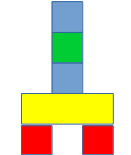
\includegraphics[width=0.25\textwidth]{figs/Chapter4/BlockGoal.png}
       \label{subfig:goal}
   }
    %~
	\subfigure[One possible initial set-up (top view)]{
        \centering
        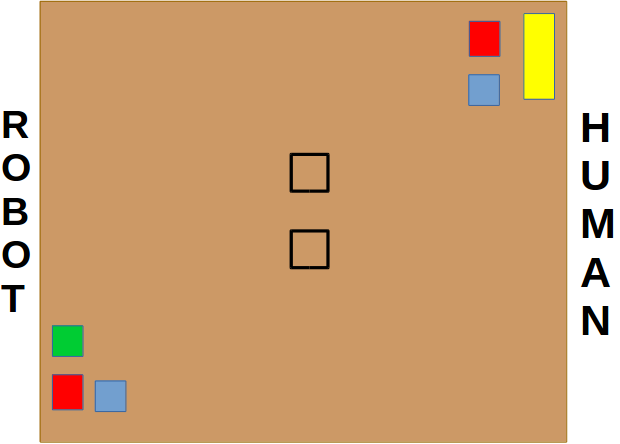
\includegraphics[width=0.4\textwidth]{figs/Chapter4/SetUp.png}
       \label{subfig:setUp}
   }
    \caption{Description of the blocks building task. The human and the robot have to build the stack together. We assume that the robot and the human know where all the available blocks are. We would like the robot to adapt as much as possible to the human actions and decisions while avoiding useless or tiresome verbal interactions}
    \label{fig:blocksBuildingTask}
\end{figure*}

\subsection{Illustrative example}

We will first present one possible scenario of the task described earlier which illustrate well the benefits of this work.

\begin{figure*}[!h]
\centering
	\subfigure[Initial plan]{
        \centering
        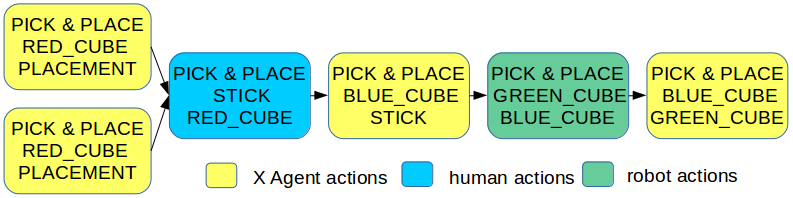
\includegraphics[width=0.7\textwidth]{figs/Chapter4/init_plan.png}
       \label{subfig:initPlan}
   }
    %~
	\subfigure[The robot chooses to put the red cube in the placement to its right]{
        \centering
        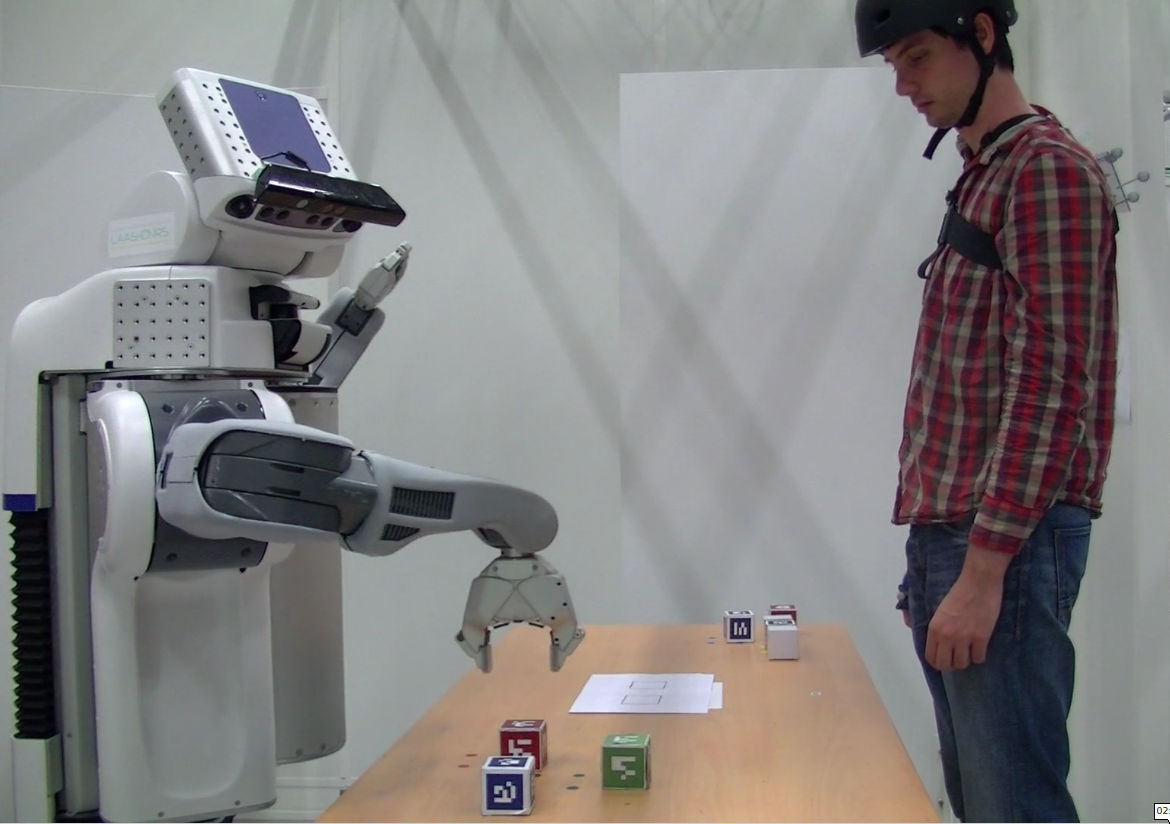
\includegraphics[width=0.4\textwidth]{figs/Chapter4/screen_shot1.jpeg}
       \label{subfig:redCube}
   }
    %~
	\subfigure[The human places his cube in the placement the robot chose]{
        \centering
        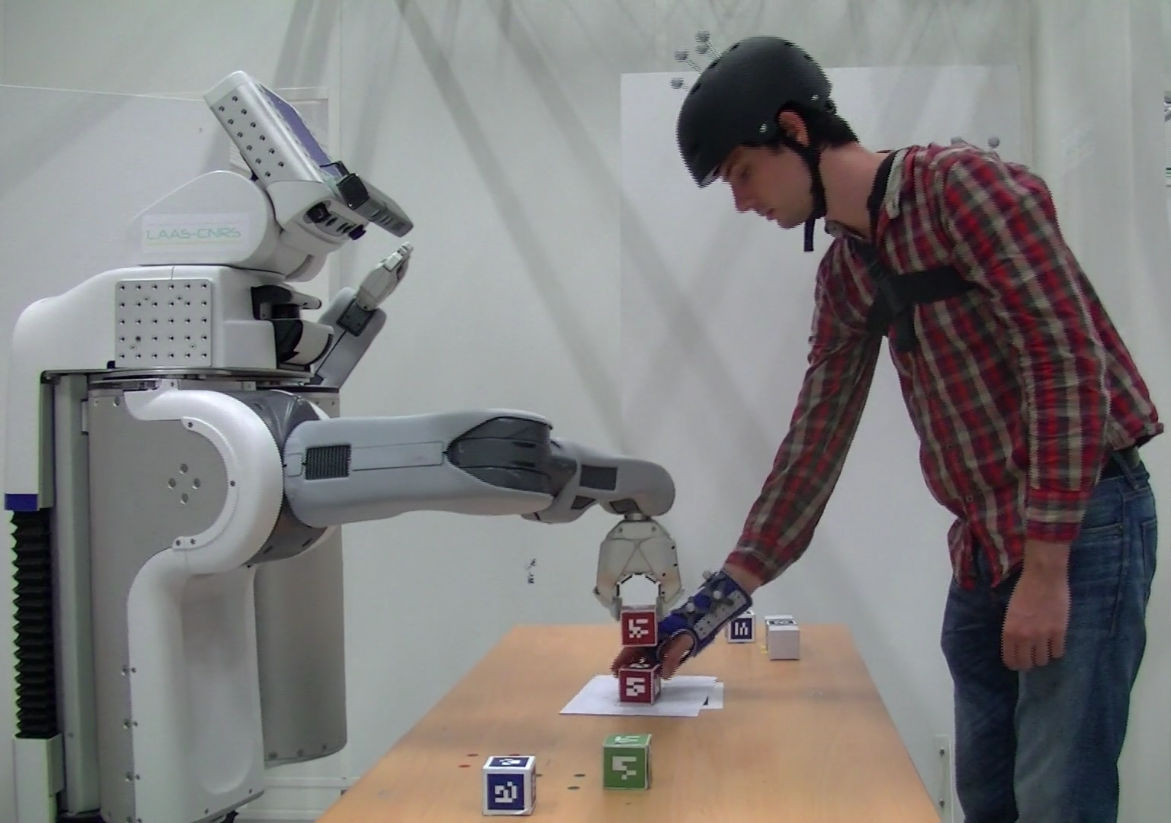
\includegraphics[width=0.4\textwidth]{figs/Chapter4/screen_shot2.jpeg}
       \label{subfig:humanPlace}
   }
    %~
	\subfigure[Second computed plan]{
        \centering
        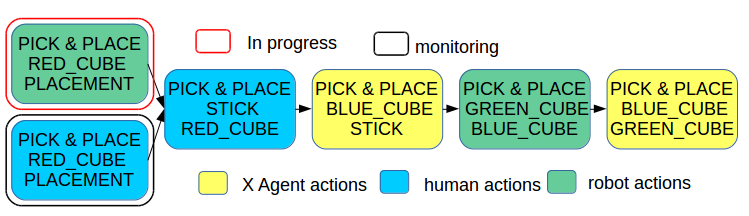
\includegraphics[width=0.7\textwidth]{figs/Chapter4/second_plan.png}
       \label{subfig:secondPlan}
   }
    %~
	\subfigure[The robot adapts by changing its placement choice]{
        \centering
        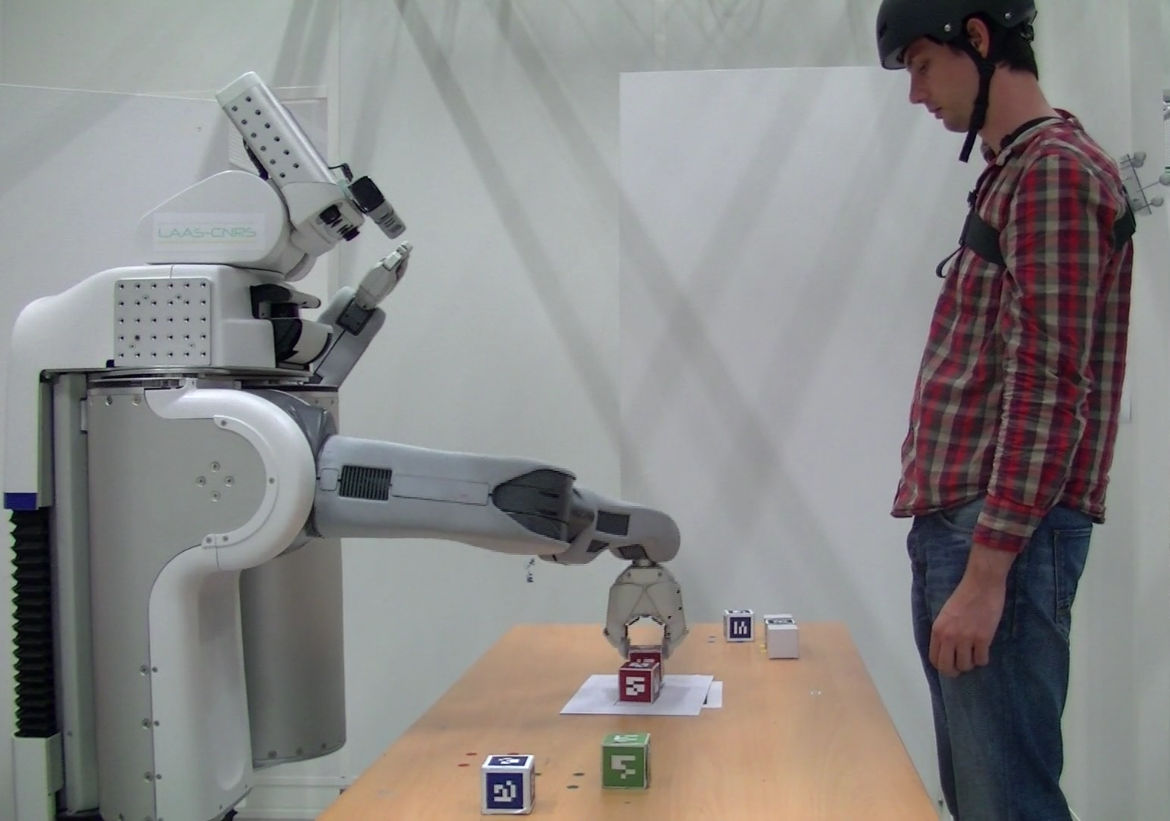
\includegraphics[width=0.4\textwidth]{figs/Chapter4/screen_shot3.jpeg}
       \label{subfig:robotAdapts}
   }
    %~
	\subfigure[Third computed plan]{
        \centering
        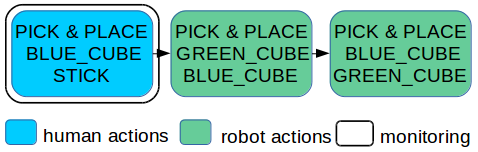
\includegraphics[width=0.4\textwidth]{figs/Chapter4/third_plan.png}
       \label{subfig:thirdPlan}
   }
    \caption{The human and the robot build a blocks construction together. The robot adapts its behavior to the human actions.}
\end{figure*}


The presented scenario starts with the set-up in Fig.~\ref{subfig:setUp}. The plan produced by HATP for this set-up can be found in Fig.~\ref{subfig:initPlan}. As this plan starts with two \textit{analogous} actions for the \textit{X agent} (place a red cube into a placement), the robot selects one and starts to execute it. So, the robot picks the red cube (Fig. \ref{subfig:redCube}) and, at the same time, looks for the consequences of its choice in the plan. As both agents own only one red cube, in the new plan computed by the robot (Fig.~\ref{subfig:secondPlan}) the human needs to place the second red cube. After picking its red cube the robot starts to place it on the placement to its right. However, the human picks his red cube and places it in the very same placement (Fig.~\ref{subfig:humanPlace}). So, the robot stops its movement and adapts by placing its cube in the other placement (Fig.~\ref{subfig:robotAdapts}). Then, the human places the stick on the red cubes. In this scenario, we have chosen to set the robot into the \textbf{negotiation} mode. As the next action is allocated to the \textit{X agent}, the robot asks the human if he wants to do it (\textit{"Do you want to place the blue cube?"}). The human answers yes, leading the robot to compute the new plan in Fig.~\ref{subfig:thirdPlan} where the human have to place the first blue cube and the robot the second one. Finally, the human and the robot perform their last actions and achieve the goal.


\subsection{Quantitative results}

In order to evaluate our system, we run it in simulation using the blocks building scenario. Different set-ups were used as initial state of the task: we randomized the number of cubes of each color in the environment and their position (accessible by the robot or the human). The robot was confronted to a simulated human with different types of behaviors. This simulated human performs all actions that are feasible only by him and answers robot questions. When confronted to an \textit{X agent} action, he either chooses to perform it with 50\% chance (50\%-case), systematically chooses to perform it (hurry-case) or systematically chooses not to perform it (lazy-case). Then, we settled two different human behaviors:
\begin{itemize}
\item \textbf{the "kind" human (case=K)} who adapts his behavior to what the robot verbalizes (ie does an action if the robot asks him and stops an action if the robot says it will perform it)
\item \textbf{the "stubborn" human (case=S)} who does not react nor comply to robot verbalization (he will not change his decision whatever the robot says).
\end{itemize}

We compared 4 different modes:
\begin{itemize}
\item using the original system, called Reference System (RS), with all decisions and instantiations performed at planning time:
\begin{itemize}
\item \textbf{RS-none mode:} the robot verbalizes nothing (unless it is strictly necessary)
\item \textbf{RS-all mode:} the robot informs the human when he has to perform an action and when it will act,
\end{itemize}
\item using the proposed system, called New System (NS): 
\begin{itemize}
\item \textbf{NS-N:} the robot uses the \textbf{Negotiation} mode previously defined when a decision need to be made concerning \textit{X agent} action,
\item \textbf{NS-A:} the robot uses the \textbf{Adaptation} mode.
\end{itemize}
\end{itemize}

We measured:
\begin{itemize}
\item \textit{the number of verbal interactions} between the human and the robot (either an information given by the robot or question asked), in Tab.~\ref{tab:incompatible}.
\item \textit{the number of human/robot incompatible decisions}: either both decide to perform the same action (and the robot stops its own action to avoid the conflict) or both decide not to perform the action (the robot first asks the human to perform the action after a predefined time and, if after another period the human has still not executed the action, the robot looks for a new plan where it can proceed), in Tab.~\ref{tab:incompatible}.
\end{itemize}
We also measured execution time but no significant difference was found between the different conditions. Indeed, this criterion is not pertinent here since, as all actions concern the same stack, they need to be performed one after the other. Consequently, there is no significant difference time between the different options.

\begin{table*}[!h]
\centering
  \begin{tabular}{|c||c|c|c|c|}
  \hline
     & \textbf{RS-none} & \textbf{RS-all} & \textbf{NS-N} & \textbf{NS-A} \\
  \hline
  \hline
     \textbf{50\%-K} & 0.6 (0.52) & & &  \\
  \cline{1-2}
     \textbf{hurry-K} & 0.3 (0.48) & 0.0 (0.0) & & \\
  \cline{1-2}
     \textbf{lazy-K} & 0.9 (0.32) &  &  &  \\
  \cline{1-3}
     \textbf{50\%-S} & 0.5 (0.53) & 0.6 (0.52) & \textbf{0.0 (0.0)} & \textbf{0.0 (0.0)} \\
  \cline{1-3}
     \textbf{hurry-S} & 0.3 (0.48) & 0.3 (0.48) &  &  \\
  \cline{1-3}
     \textbf{lazy-S} & 0.9 (0.32) & 0.9 (0.32) &  &  \\
  \hline
  \end{tabular}
   \caption{Results for the reference system (RS) and the proposed system (NS-N for the negotiation mode and NS-A for the adaptation mode). Number of incompatible decisions between the human and the robot (i.e. either both agents decide to perform the same action or both decide not to perform a given action). The numbers correspond to means in 10 runs and their associated standard deviations.}
   \label{tab:incompatible} 
\end{table*}


\begin{table*}[!h]
\centering
  \begin{tabular}{|c||c|c|c|c|}
  \hline
     & \textbf{RS-none} & \textbf{RS-all} & \textbf{Neg} & \textbf{Adapt} \\
  \hline
  \hline
     \textbf{50\%-K} & 0.4 (0.52) &  &  &  \\
  \cline{1-2}
     \textbf{hurry-K} & 0.0 (0.0) & 6.0 (0.0) & &  \\
  \cline{1-2}
     \textbf{lazy-K} & 0.9 (0.32) &  &  &  \\
  \cline{1-3}
     \textbf{50\%-S} & 0.4 (0.52) & 6.4 (0.52) &\textbf{ 1.2 (0.0)} & \textbf{0.0 (0.0)} \\
  \cline{1-3}
     \textbf{hurry-S} & 0.0 (0.0) & 6.0 (0.0) &  & \\
  \cline{1-3}
     \textbf{lazy-S} & 0.9 (0.32) & 6.9 (0.32) & & \\
  \hline
  \end{tabular}
   \caption{Results for the reference system (RS) and the proposed system (NS-N for the negotiation mode and NS-A for the adaptation mode). Number of verbal interactions (i.e. question asked by the robot in the negotiation mode or an information given with the reference system). The numbers correspond to means in 10 runs and their associated standard deviations.}
   \label{tab:verb}
\end{table*}


\paragraph{Reference System performance:} 
The verbalizations in the RS-none mode corresponds to the case where the human and the robot both choose not to execute the action: the robot tries to solve the conflict by asking the human to execute the action. Because the robot does not inform about its decisions, the number of verbal interactions is low in this mode. However, due to the same reason, there is several incompatible decisions in each conditions. The RS-all mode avoids incompatible decisions with the "kind" human. However, the number of verbal interaction is high (6 as the number of actions to execute in the task and so to verbalize). With the "stubborn" human, even if the robot informs the human, incompatible decisions remains. The number of verbal interaction also increases as, when the human does not want to perform the action, as it is stubborn, the robot needs to compute a new plan where it executes the action, and so inform about the new action.

\paragraph{New System performance:} We can see that the robot is able to avoid conflicts in all cases without being too talkative (or without being talkative at all for the adaptation mode). Moreover, the efficiency of the system is not degraded with the "stubborn" human: the system allows the human to execute the actions he wants without an increase of verbal interaction. 
Finally, here the adaptation mode performs better than the negotiation one since the human is simulated and always performs his actions in time. However, in a real context, the negotiation mode would certainly have the benefit to ensure the absence of conflicts even if the robot is a little more talkative. Moreover, a human would surely be more comfortable with a robot which directly asks when (and only when) there is a decision to take compared to a robot which has unnecessary waiting time. Such measure of "satisfaction" cannot be easily simulated and further experiments will be done with real humans.

\section{Conclusion}

In this chapter we shown how we enable the robot to compute and execute more flexible Shared Plans. In these new plans, the needed decisions on who will execute an action and with which objects are let to the execution. A number of the presented algorithms involve cost estimation in order to decide between options. In the current system, simple costs are used but could be easily replaced by more elaborate ones. For instance, a finer estimation of action costs based on geometric reasoning and human efforts would allow better informed choice for action or object selection. Another interesting issue would be to integrate the estimation of accumulated costs of all actions remaining in the plan.

The benefits of this work have been demonstrated with an illustrative example and simulation results. We will show in Chapter~\ref{ch:Eval}) more complete simulation results which also include the work of the previous chapter as well as results with the system running in a real situation.


\ifdefined\included
\else
\bibliographystyle{StyleThese}
\bibliography{These}
\end{document}
\fi
